\chapter{Introduction to Binary Classification}

The problem of data classification is very important mathematical problem. The goal of classification is to find a relation between a set of objects and a target variable based on some properties of the objects. The properties of the objects are usually called features. There are many problems in research as well as in the real world that can be formulated as classification tasks. We can find applications of data classification across all the fields:
\begin{itemize}
  \item \textbf{Medical Diagnonsis:} In medicine, the classification is often used to improve disease diagnosis. In such a case, the features are medical records such as the patient's blood tests, temperature, or roentgen images. The target variable is if the patient has some disease. As an example, classification is used to process mammogram images and detect cancer~\cite{viale2012current, levy2016breast}.
  \item \textbf{Internet Secutiry:} These days, the internet is a crucial part of our lives. With the increasing usage of the internet, the number of attacks increases as well. An essential part of the defense are intrusion detection systems~\cite{grill2016learning, scarfone2007guide} that search for malicious activities (network attacks) in network traffic. Classification can be used to improve such systems~\cite{giacinto2002intrusion, shanbhag2009accurate}.
  \item \textbf{Marketing:} In marketing, the task can be to classify customers based on their buying interests. Such information can be used to build a personalized recommendation system for customers and therefore increase income~\cite{kaefer2005neural, zhang2007building}.
\end{itemize}
Many other classification problems can be found in almost all fields. Also, there is a vast number of classification algorithms that try to solve these classifications problems. Typically these algorithms consist of two phases:
\begin{itemize}
  \item \textbf{Training Phase:} In the training phase, the algorithm uses training data to build a model. The classification algorithms fall into the category of supervised learning algorithms. It means, that these algorithms must have labeled training data to build the model, i.e. the algorithm must have the knowledge of the target classes. The training data typically consists of pairs (sample, label) and can be described as follows
  \begin{equation*}\label{eq: training set}
    \D_{\mathrm{train}} = \Brac[c]{(\bm{x}_i, y_i)}_{i=1}^{n},
  \end{equation*}
  where the sample~$\bm{x}_i \in \R^d$ is a~$d$-dimensional vector of features that describes the object of interes and the label~$y_i \in \{1, 2, \ldots, k\}$ represents target class. Moreover~$n \in \N$ is a number of training samples and~$k \in \N$ is a number of target classes.
  \item \textbf{Testing Phase:} In the testing phase, the model is used to assign labels~$\hat{y}_i \in \{1, 2, \ldots, k\}$ to the data from testing set which was not known during the training phase
  \begin{equation*}\label{eq: test set}
    \D_{\mathrm{test}} = \Brac[c]{(\bm{x}_i, y_i)}_{i=1}^{m},
  \end{equation*}
  where~$\bm{x}_i \in \R^d,$~$y_i \in \{1, 2, \ldots, k\}$ and~$m \in \N$ is a number of testing samples. The ultimate goal of all classification algorithms is to classify testing samples with the highest accuracy possible.
\end{itemize}
The previous definitions of training and test set are general for classification problems with multiple classes. However, the main focus of this work is on a special subclass of classification problems with only two target classes: binary classification. The binary classification is a special case of classification in which the number of classes is~$k=2.$ These two classes are usually referred to as negative and positive classes and the positive class is the one that we are more interested in. If we go back to the mammogram example, the positive class would represent cancer. The positive class is usually encoded using label~$1.$ The encoding of the negative class differs for different algorithms. For example, SVM-like algorithms (from Support Vector Machines~\cite{cortes1995support}) usually use the label~$-1$ for the negative class. On the other hand, neural networks usually use the label~$0$ for the negative class. 

\begin{notation}[Dataset]\label{eq: dataset}
  In the rest of the work,, we follow the notation used for neural networks, i.e. we use~$1$ as positive label and~$0$ as negative label. Moreover, by dataset of size~$n \in \N$ we mean set in the form
  \begin{equation*}\label{eq: train set bin}
    \D = \Brac[c]{(\bm{x}_i, y_i)}_{i=1}^{n},
  \end{equation*}
  where~$\bm{x}_i \in \R^d$ represents samples,~$d \in \N$ its dimension and~$y_i \in \{0, 1\}$ represents corresponding labels. To simplify future notation, we denote set of all indices of dataset~$\D$ as~$\I = \I^- \cup \I^+,$ where
  \begin{equation*}
    \begin{aligned}
      \I^- & = \Set{i}{i \in \{1, 2, \ldots, n\} \; \land \; y_i = 0}, \\
      \I^+ & = \Set{i}{i \in \{1, 2, \ldots, n\} \; \land \; y_i = 1}.
    \end{aligned}
  \end{equation*}
  We also denote the number of negative samples in~$\D$ set as~$n^- = \Brac[v]{\I^-}$ and the number of positive samples in~$\D$ as~$n^+ = \Brac[v]{\I^+},$ i.e. total number of samples is~$n = n^- + n^+.$ 
\end{notation}

\section{General Formulation}\label{sec: general formulation}

Generally, the problem of binary classification can be written as follows
\begin{mini}{\bm{w}, t}{
    \lambda_1 \sum_{i \in \I^-} \Iverson{s_i \ge t} + \lambda_2 \sum_{i \in \I^+} \Iverson{s_i < t}
  }{\label{eq: Binary classification}}{}
  \addConstraint{s_i}{= f(\bm{x}_i; \bm{w}), \quad}{i \in \I,}
\end{mini}
where~$\lambda_1, \lambda_2 \in \R,$ the function~$f \colon \R^d \to \R$ represents the model and maps samples~$\bm{x}_i$ to classification scores~$s_i$ and~$\Iverson{\cdot{}}$ represents Iverson function that is used to counts misclassified samples and is defined as
\begin{equation}\label{eq: iverson}
  \Iverson{x} = \begin{cases}
    0 & \text{if } x \text{ is false}, \\
    1 & \text{if } x \text{ is true}. \\
  \end{cases}
\end{equation}
Moreover, the vector~$\bm{w} \in \R^d$ represents trainable parameters (weights) of the model~$f$ and~$t \in R$ is a decision threshold. The parameters~$\bm{w}$ are determined from training data during the training phase of classification algorithm. Although the decision threshold~$t$ can also be determined from the training data, in many cases it is fixed. For example, for many algorithms the classification score~$s_i$ given by the model~$f$ represents the probability that the sample~$\bm{x}_i$ belongs to the positive class. Therefore, it makes sense to set the decision threshold to~$t = 0.5$ and classify the sample as positive if its classification score is larger than this threshold.

\todo[inline]{Add definition of classification scores and describe model weights (parameters).}

\begin{notation}[Classifier]\label{eq: classifier}
  By classifier, we always mean pair of model~$f \colon \R^d \to \R$ which maps~$\bm{x}$ to classification scores~$s$ and corresponding decision threshold~$t \in \R$. Prediction~$\hat{y}$ for the given classifier is define as follows
  \begin{equation*}
    \hat{y} = \begin{cases}
      1 \ldots & \text{if } f(\bm{x}; \bm{w}) \ge t, \\
      0 \ldots & \text{otherwise.}
    \end{cases}
  \end{equation*}
\end{notation}

\section{Performance Evaluation}

In the previous section we defined general binary classification problem~\ref{eq: Binary classification}. However, we did not discuss yet how to measure the performance of the resulting classifier. In this section, we will introduce basic approaches that are used to measure the performance of binary classifiers.

\subsection{Confusion Matrix}
Based on the prediction~$\hat{y}_i$ and an actual label~$y_i$ of the sample~$\bm{x}_i,$ each sample can be assigned to one of the following categories
\begin{itemize}
  \item \textbf{True negative:}~$\bm{x}_i$ is negative and is classified as negative, i.e.~$y_i = 0 \; \land \; \hat{y}_i = 0.$
  \item \textbf{False positive:}~$\bm{x}_i$ is negative and is classified as positive, i.e.~$y_i = 0 \; \land \; \hat{y}_i = 1.$
  \item \textbf{False negative:}~$\bm{x}_i$ is positive and is classified as negative, i.e.~$y_i = 1 \; \land \; \hat{y}_i = 0.$
  \item \textbf{True positive:}~$\bm{x}_i$ is positive and is classified as positive, i.e.~$y_i = 1 \; \land \; \hat{y}_i = 1.$
\end{itemize}
Using these four categories, we can construct a so-called confusion matrix (sometimes also called contingency table)~\cite{fawcett2006introduction} that represents the results of predictionS for all samples from the given dataset~$\D$. An illustration of the confusion matrix is shown in Figure~\ref{fig: confusion matrix}. If we denote vector classification scores given by model~$f$ as~$\bm{s} \in \R^n,$ where~$s_i = f(\bm{x}_i; \bm{w})$ for all~$i \in \I,$ we can compute all fields of the confusion matrix as follows
\begin{equation}\label{eq: confusion counts}
  \begin{aligned}
    \tp(\bm{s}, t) & = \sum_{i \in \I^+}\Iverson{s_i \ge t}, & \quad
    \fn(\bm{s}, t) & = \sum_{i \in \I^+}\Iverson{s_i < t}, \\
    \tn(\bm{s}, t) & = \sum_{i \in \I^-}\Iverson{s_i < t}, & \quad
    \fp(\bm{s}, t) & = \sum_{i \in \I^-}\Iverson{s_i \ge t}.
  \end{aligned}
\end{equation}
In the following text, we will sometimes use simplified notation~$\tp = \tp(\bm{s}, t)$ (similarly fo the other counts) for example to define classification metrics. In such cases, the vector of classification scores and decision threshold is fixed and is known from the context. Using the simplified notation we can simply define true-positive, false-positive, true-negative and false-negative rates as follows
\begin{equation}\label{eq: confusion rates}
  \begin{aligned}
    \tpr & = \frac{\tp}{n^{+}}, & \quad
    \fnr & = \frac{\fn}{n^{+}}, & \quad
    \tnr & = \frac{\tn}{n^{-}}, & \quad
    \fpr & = \frac{\fp}{n^{-}}. \\
  \end{aligned}
\end{equation}
Figure~\ref{fig: scores and rates} show the relation between these for classification rates and the classification scores and the decision threshold. The blue and red curves represent theoretical distribution of the scores of negative and positive samples samples respectively. The position of the decision threshold determines the values of the classification rates. The higher the value of the decision threshold, the smaller the false-positive rate, but at the same time the higher the false-negative rate. Similarly, the smaller the value of the decision threshold, the higher the false-positive rate and the smaller the false-negative rate. Ideally, classification without errors is the goal, but it is not usually possible and therefore we have to try to find some trade-off between false positive and a false negative rate. There is no universal truth, which error is worse. For example, we may want to detect cancer from some medical data. In this case, it is probably better to classify a healthy patient as sick than the other way around. On the other hand, in the computer security we do not want an antivirus program that makes a lot of false-positive alerts since it will be disruptive for the user. If we get look at the general definition of the binary classification problem~\eqref{eq: Binary classification}, we can see, that the objective function is in fact just the weighted sum of false positive and false negative samples, i.e. we can use the notation~\eqref{eq: confusion rates} and rewrite the problem~\eqref{eq: Binary classification} to the following form
\begin{mini}{\bm{w}, t}{
    \lambda_1 \cdot \fp(\bm{s}, t) + \lambda_2 \cdot \fn(\bm{s}, t)
  }{\label{eq: Binary classification counts}}{}
  \addConstraint{s_i}{= f(\bm{x}_i; \bm{w}), \quad}{i \in \I.}
\end{mini}
The parameters~$\lambda_1, \; \lambda_2 \in \R$ are used to specify which error is more serious for the particular classification task.

\begin{figure}
  \centering
  \begin{NiceTabular}{cccccc}[cell-space-limits = 7pt]
    && \Block[draw=black, line-width=2pt, rounded-corners]{1-2}{
      \longcell{\textbf{Predicted label}}
    } \\
    && $\hat{y} = 0$
    &  $\hat{y} = 1$
    && \Block{1-1}{\textbf{Row total:}} \\
    \Block[draw=black, line-width=2pt, rounded-corners]{2-1}{
      \rotate \longcell{\textbf{Actual} \\ \textbf{label}}
    }
    & $y = 0$
    & \Block[draw=mygreen, fill=mygreen!50, rounded-corners]{1-1}{
      \longcell{true \\ negatives \\ (\textbf{tn})}
    }
    & \Block[draw=myred, fill=myred!50, rounded-corners]{1-1}{
      \longcell{false \\ positives \\ (\textbf{fp})}
    }
    & $\rightarrow$
    & \Block[draw=black, rounded-corners]{1-1}{\longcell{all \\ negatives \\ ($n^{-}$)}} \\
    & $y = 1$
    & \Block[draw=myred, fill=myred!50, rounded-corners]{1-1}{
      \longcell{false \\ negatives \\ (\textbf{fn})}
    }
    & \Block[draw=mygreen, fill=mygreen!50, rounded-corners]{1-1}{
      \longcell{true \\ positives \\ (\textbf{tp})}
    }
    & $\rightarrow$
    & \Block[draw=black, rounded-corners]{1-1}{\longcell{all \\ positives \\ ($n^{+}$)}} \\
    && $\downarrow$
    &  $\downarrow$ \\
    \Block{1-2}{\longcell{\textbf{Column} \\ \textbf{total:}}}
    && \Block[draw=black, rounded-corners]{1-1}{
      \longcell{all predicted \\ negatives}
    }
    & \Block[draw=black, rounded-corners]{1-1}{
      \longcell{all predicted \\ positives}
    }
  \end{NiceTabular}
  \caption{Representation of the confusion matrix for the binary classification problem, where the negative class has label~$0$ and the positive class has label~$1.$ The true (target) label is denoted as~$y$ and predicted label is denoted as~$\hat{y}.$}
  \label{fig: confusion matrix}
\end{figure}

\begin{figure}
  \centering
  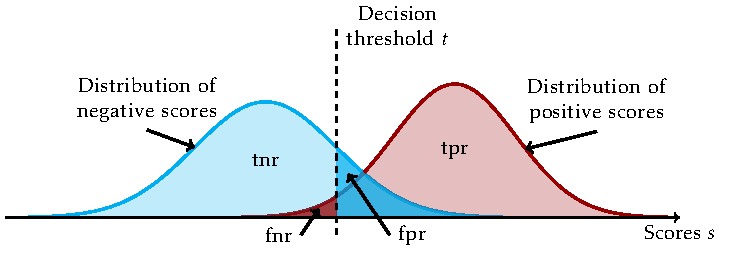
\includegraphics[width=\linewidth]{images/confusion_rates.pdf}
  \caption{The relation between classification scores and  rates. The blue curve represents theoretical distribution of the scores of negative samples and the red curve the same for the score of positive samples. Filled areas with light blue or red color represent true-negative and true-positive rates respectively. Similarly the filled areas with dark blue or red color represent false-positive and false-negaives rates.}
  \label{fig: scores and rates}
\end{figure}
In addition to the confusion matrix, there are many other classification metrics, and many of them are derived directly from the confusion matrix. As an example, we can mention accuracy and the balanced accuracy. Accuracy is defined as the ratio of correctly classified samples from all samples~\cite{metz1978basic}
\begin{equation*}
  \accuracy = \frac{\tp + \tn}{n}.
\end{equation*}
However, the accuracy is not suitable for unbalanced datasets, i.e. for dataset where the number of samples in one class is significantly higher then the number of samples in the other class. In such a case, the balanced accuracy is better. The balanced accuracy is defined as an average of true-positive and true-negative rate~\cite{brodersen2010balanced}
\begin{equation*}
  \baccuracy = \frac{1}{2}\Brac{\tpr + \tnr}.
\end{equation*}
The difference can be easily demonstrated on a simple example. Let us suppose that we have 100 samples and 10 of them is negatives and the rest is positive. If we use simple classifier that all samples clasify as positive we will get the following accuracy
\begin{equation*}
  \accuracy = \frac{90 + 0}{100} = 0.9.
\end{equation*}
Even though we know, that the classifier totally ignores negative samples, the accuracy is still 90\%. The reason is, that the used classifier is biased towards the more frequent class. Balanced accuracy solves this problem by using true-positive and true-negative rates instead of counts, which leads to the following results for the given example
\begin{equation*}
  \baccuracy = \Brac{\frac{90}{90} + \frac{0}{10}} = 0.5.
\end{equation*}
In this case the balanced accuracy is only 50\% which is very poor, but is more relevant to the unbalanced dataset. There are many more classification metrics that are based on the confusion matrix~\cite{fawcett2006introduction, metz1978basic, brodersen2010balanced, hossin2015review}. In this work, however, we will use mainly those that we have presented in this section.

\begin{table}
  \centering
  \begin{NiceTabular}{ccc}
    \toprule
    \textbf{Name} & \textbf{Aliases} & \textbf{Formula} \\
    \midrule
    true negatives
      & correct rejection
      & $\tn$ \\
    false positives
      & Type I error, false alarm
      & $\fp = n^- - \tn$ \\
    true positives
      & hity
      & $\tp$ \\
    false negatives
      & Type II error
      & $\fn = n^+ - \tp$ \\
    \midrule
    true negative rate
      & specificity, selectivity
      & $\tnr = \frac{\tn}{n^-}$ \\
    false positive rate
      & fall-out
      & $\fpr = \frac{\fp}{n^-} = 1 - \tnr$ \\
    true positive rate
      & sensitivity, recall, hit rate
      & $\tpr = \frac{\tp}{n^+}$ \\
    false negative rate
      & miss rate
      & $\fnr = \frac{\fn}{n^+} = 1 - \tpr$ \\
    \midrule
    accuracy
      & ---
      & $\accuracy = \frac{\tp + \tn}{n}$ \\
    balanced accuracy
      & ---
      & $\baccuracy = \frac{\tpr + \tnr}{2}$ \\
    precision
      & positive predictive value
      & $\precision = \frac{\tp}{\tp + \fp}$ \\
    \bottomrule
  \end{NiceTabular}
  \caption{Classicication metrics}
  \label{tab: classification metrics}
\end{table}

\subsection{ROC Analysis}

In the previous section, we defined general binary clasification problem as a minimization task with objective that consists of a weighted sum of the false-positive and false-negative counts~\eqref{eq: Binary classification counts}. For fixed model~$f$ and decision threshold~$t$, the results can be visualized in the Receiver Operating Characteristic space~\cite{egan1975signal}.

\todo[inline]{Finish roc section}

\section{Related Problems}

The aim of classical binary classification is to separate positive and negative samples with the highest possible accuracy. However, in many applications, it is desirable to separate only a certain number of samples. In such a case, the goal is not to maximize the performance on all samples but only the performance on the required samples with the highest relevance. The rest of the samples is irrelevant and therefore the performance on them is not important. Figure~\ref{fig: standard vs. aatp} shows the difference between the standard classifier (classifier 1) that maximizes the accuracy and the classifier that focuses only on the classification at the top (classifier 2). In this particular case, the classifier 2 tries to maximize the number of positive samples that are ranked higher than the worst negative sample, i.e. the negative sample with the highest score. Formally, we can define metric
\begin{equation*}
  \postop(\bm{s}) = \frac{1}{n^+} \sum_{i \in \I^+} \Iverson{s_i \ge \max_{j \in \I^-}\{s_j\}}.
\end{equation*}
While classifier 1 has good total~$\accuracy$, its~$\postop$ metric is subpar because of the few negative outliers. On the other hand, classifier 2 has worse total~$\accuracy$, but its~$\postop$ metric is extremely good because more than half of the positive samples are ranked higher than the worst negative sample. While classifier 1 selected different thresholds for the~$\accuracy$ and~$\postop$ metrics, these thresholds coincide for classifier 2. In the rest of the chapter, we will present three main categories of problems that are closely related to the binary classification but do not focus on optimizing overall performance.

\begin{figure}[t]
  \centering
  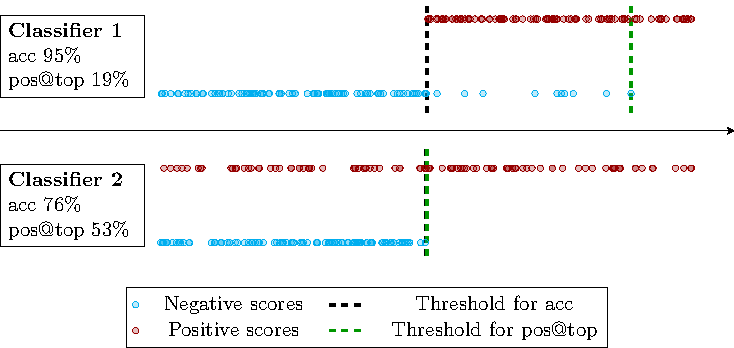
\includegraphics[width = \linewidth]{images/standard_aatp_comparison.pdf}
  \caption{Difference between standard classifiers (\textbf{Classifier~1}) and classifiers maximizing~$\postop$ metric (\textbf{Classifier~2}). While the former has a good total~$\accuracy$, the latter has a~$\postop$ metric.}
  \label{fig: standard vs. aatp}
\end{figure}

\subsection{Ranking problems}

\textbf{Ranking problems:} Ranking problems~\cite{freund2003efficient, agarwal2011infinite, rudin2009pnorm, li2014top} select the most relevant samples and rank them. To each sample, a numerical score is assigned, and the ranking is performed based on this score. Often, only scores above a threshold are considered. As an example, we can mention search engines such as Google, DucDucGo or Yahoo. In such a case, the goal is to provide most relevant results on the first two or three pages. The results on page 50 are usually of no interest to anyone, so it is important to move the most relevant results to the few first pages~\cite{cortes2003auc}.

The first category of problems that is tightly related to binary classification at the top, is the category of ranking problems. Ranking problems have become very important in many different fields
\begin{itemize}
  \item \textbf{Information retrieval systems:} The goal of the information retrieval systems is to rank documents according to relevance to a given query.
  \item \textbf{Recommendation  systems:} The goal is to rank and recommend products based on the user's previous behavior.
  \item 
\end{itemize}
All the examples above can be formulated as bipartite ranking problem~\cite{freund2003efficient, agarwal2005generalization, agarwal2011infinite}, where the goal is to rank the relevant (positive) samples higher than the non-relevant (negative) ones. 

Ranking problems~\cite{freund2003efficient, agarwal2011infinite, rudin2009pnorm, li2014top} select the most relevant samples and rank them. To each sample, a numerical score is assigned, and the ranking is performed based on this score. Often, only scores above a threshold are considered. As an example, we can mention search engines such as Google, DucDucGo or Yahoo. In such a case, the goal is to provide most relevant results on the first two or three pages. The results on page 50 are usually of no interest to anyone, so it is important to move the most relevant results to the few first pages~\cite{cortes2003auc}.

A prototypical example is the RankBoost~\cite{freund2003efficient} maximizing the area under the ROC curve, the Infinite Push~\cite{agarwal2011infinite} or the~$p$-norm push~\cite{rudin2009pnorm} which concentrate on the high-ranked negatives and push them down. Since all these papers include pairwise comparisons of all samples, they can be used only for small datasets. This was alleviated in~\cite{li2014top}, where the authors performed the limit~$p \to \infty$ in~$p$-norm push and obtained the linear complexity in the number of samples. Moreover, since the~$l_{\infty}$-norm is equal to the maximum, this method falls into our framework with the threshold equal to the largest score computed from negative samples.

Many methods, such as \emph{RankBoost}~\cite{freund2003efficient}, \emph{Infinite Push}~\cite{agarwal2011infinite} or \emph{$p$-norm push}~\cite{rudin2009pnorm} employ a pairwise comparison of samples, which makes them infeasible for larger datasets. This was alleviated in \TopPush~\cite{li2014top} where the authors considered the limit~$p \rightarrow \infty$. Since the~$l_{\infty}$ norm from \TopPush is equal to the maximum, the decision threshold from our framework equals to the maximum of scores of negative samples. This was generalized into \TopPushK~\cite{adam2021general} by considering the threshold to be the mean of~$K$ largest scores of negative samples.

\subsection{Accuracy at the Top}

\textbf{Accuracy at the Top:} Accuracy at the Top~\cite{boyd2012accuracy, grill2016learning} is similar to ranking problems. However, instead of ranking the most relevant samples, it only maximizes the number of positive samples (equivalently minimizes the misclassification)  above the top~$\tau$-quantile of scores. The Accuracy at the Top can be very useful for search engines or in applications where identified samples undergo expensive post-processing such as human evaluation. As an example, we can mention cyber security~\cite{grill2016learning}, where a low false-negative rate is crucial as a high number of false alarms would result in the software being uninstalled, or drug development, where potentially useful drugs need to be preselected and manually investigated.

Accuracy at the Top ($\tau$-quantile) was formally defined in~\cite{boyd2012accuracy} and maximizes the number of relevant samples in the top~$\tau$-fraction of ranked samples. When the threshold equals the top~$\tau$-quantile of all scores, this problem falls into our framework. The early approaches aim at solving approximations, for example,~\cite{joachims2005svm} optimizes a convex upper bound on the number of errors among the top samples. Due to the presence of exponentially many constraints, the method is computationally expensive.~\cite{boyd2012accuracy} presented an SVM-like formulation which fixes the index of the quantile and solves~$n$ problems. While this removes the necessity to handle the (difficult) quantile constraint, the algorithm is computationally infeasible for a large number of samples.~\cite{kar2015surrogate} derived upper approximations, their error bounds and solved these approximations.~\cite{grill2016learning} proposed the projected gradient descent method where after each gradient step, the quantile is recomputed.~\cite{eban2017scalable} suggested new formulations for various criteria and argued that they keep desired properties such as convexity.~\cite{tasche2018plug} showed that accuracy at the top is maximized by thresholding the posterior probability of the relevant class. The closest approach to our framework is~\cite{lapin2015top,lapin2018analysis}, where the authors considered multi-class classification problems, and their goal was to optimize the performance on the top few classes and~\cite{mackey2018constrained}, where the authors implicitly removed some variables and derived an efficient algorithm.

\AccatTop~\cite{boyd2012accuracy} focuses on maximizing the number of positive samples above the top~$\tau$-quantile of scores. There are many methods on how to solve accuracy at the top. In~\cite{boyd2012accuracy}, the authors assume that the top quantile is one of the samples, construct~$n$ unconstrained optimization problems with fixed thresholds, solve them and select the best solution. This method is computationally expensive. In~\cite{grill2016learning} the authors propose a fast projected gradient descent method. In our previous paper, we proposed a convex approximation of the accuracy at the top called \PatMat. This method is reasonably fast and guaranteed the existence of global optimum.

\subsection{Hypothesis Testing}

\textbf{Hypothesis testing} states a null and an alternative hypothesis. The Neyman-Pearson problem minimizes the Type II error (the null hypothesis is false but it fails to be rejected) while keeping the Type I error (the null hypothesis is true but is rejected) small. If the null hypothesis states that a sample has the positive label, then Type II error happens when a positive sample is below the threshold and thus minimizing the Type II error amounts to minimizing the positives below the threshold.

Hypothesis testing states a null and an alternative hypothesis. The Neyman-Pearson problem minimizes the Type II error (the null hypothesis is false but it fails to be rejected) while keeping the Type I error (the null hypothesis is true but is rejected) small. If the null hypothesis states that a sample has the positive label, then Type II error happens when a positive sample is below the threshold and thus minimizing the Type II error amounts to minimizing the positives below the threshold.